\documentclass[main.tex]{subfiles}


\begin{document}

\begingroup

\renewcommand{\cleardoublepage}{}

\renewcommand{\clearpage}{}
\newpage
\chapter{Perception Function Documentation}

\section{Introduction}
\chapterauthor{Jan-Frederik Stock}
The task of the perception group was to use the available image data to gather as much information as possible about the perceived scene. In the following chapter the tools and software used and created by the perception group will be described. These include descriptions of the pipelines and annotators used in RoboSherlock, the image processing framework used by the perception group, as well as tools for classification.

\section{RoboSherlock}
		\chapterauthor{Jan-Frederik Stock}
The main framework the perception group is working with is RoboSherlock \footnote{\url{http://www.robosherlock.org/}}. RoboSherlock is a software, that uses multiple expert systems called annotators on input image data. Each annotator performs a specific task, for example searching for objects in a given picture. All annotators write their results to a public data structure.\\
		
RoboSherlock works by executing all of these annotators in a predefined order. This order is called a pipeline. There can be pipelines for different purposes, in the perception groups case for detecting objects and detecting surfaces. Each pipeline can have different annotators. Thus, RoboSherlock can be customized to achieve many different image processing tasks.

		\section{rs\_perception}
		\chapterauthor{Leonidas Paniago}
			\subsection{Pipeline: hsrb\_1ms}

The main pipeline for detecting and identifying objects with RoboSherlock consists of the following annotators:  
\begin{itemize}
	\item CollectionReader : Takes care of the Camera  Input
	\item ImagePreprocessor : Create missing Images and implement Image Filters  
	\item SuturoRegionFilter : Remove all points that are not in the defined Regions 
	\item NormalEstimator : Estimate Surface Normals in a PointCloud 
	\item PlaneAnnotator : Search for Horizontal Planes in which the search location for Objects is set
	\item PointCloudClusterExtractor : Extract all Points found in the PointCloud that are perpendicular to the Plane 
	\item ClusterColorHistogramCalculator : Calculate the individual color quantity in relation to all colors on the cluster   
	\item Cluster3DGeometryAnnotator : Extracts basic attributes of cluster like initial pose, semantic size and 3D bounding box 
	\item SuturoShapeAnnotator : Detects the shape of the object (cylinder, sphere, box)
	\item RegionAnnotator : Further restriction on which areas will be used based on defined Regions 
	\item CaffeAnnotator : Deep learning method for Object recognition based on prerecorded Images 
	\item KnnAnnotator : Uses K-Nearest-Neighbor for classification of Objects 
\end{itemize}

Each annotator contains a changeable parameter that enables customization to the given tasks.
A \textit{RoboSherlock} pipeline works sequentially meaning any change to the order of the annotators can change the result. Some of the annotators are essential for the pipeline to work, like the CollectionReader or PlaneAnnotator, which must be executed before the other annotators. 
The following pictures are an example of the hsrb\_1ms pipeline output in exact order:  \\
%Bild Hinzufügen 

\begin{figure}[H]
\centering
%
        \subfigure[ImagePreProcessor]{%
            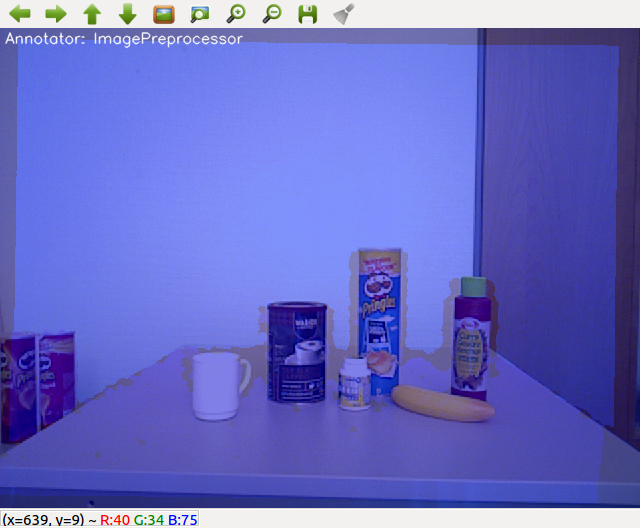
\includegraphics[width=0.5\textwidth]{pictures/2d/ImagePreProcessor.png}
        }%
        \subfigure[SuturoRegionFilter]{%
           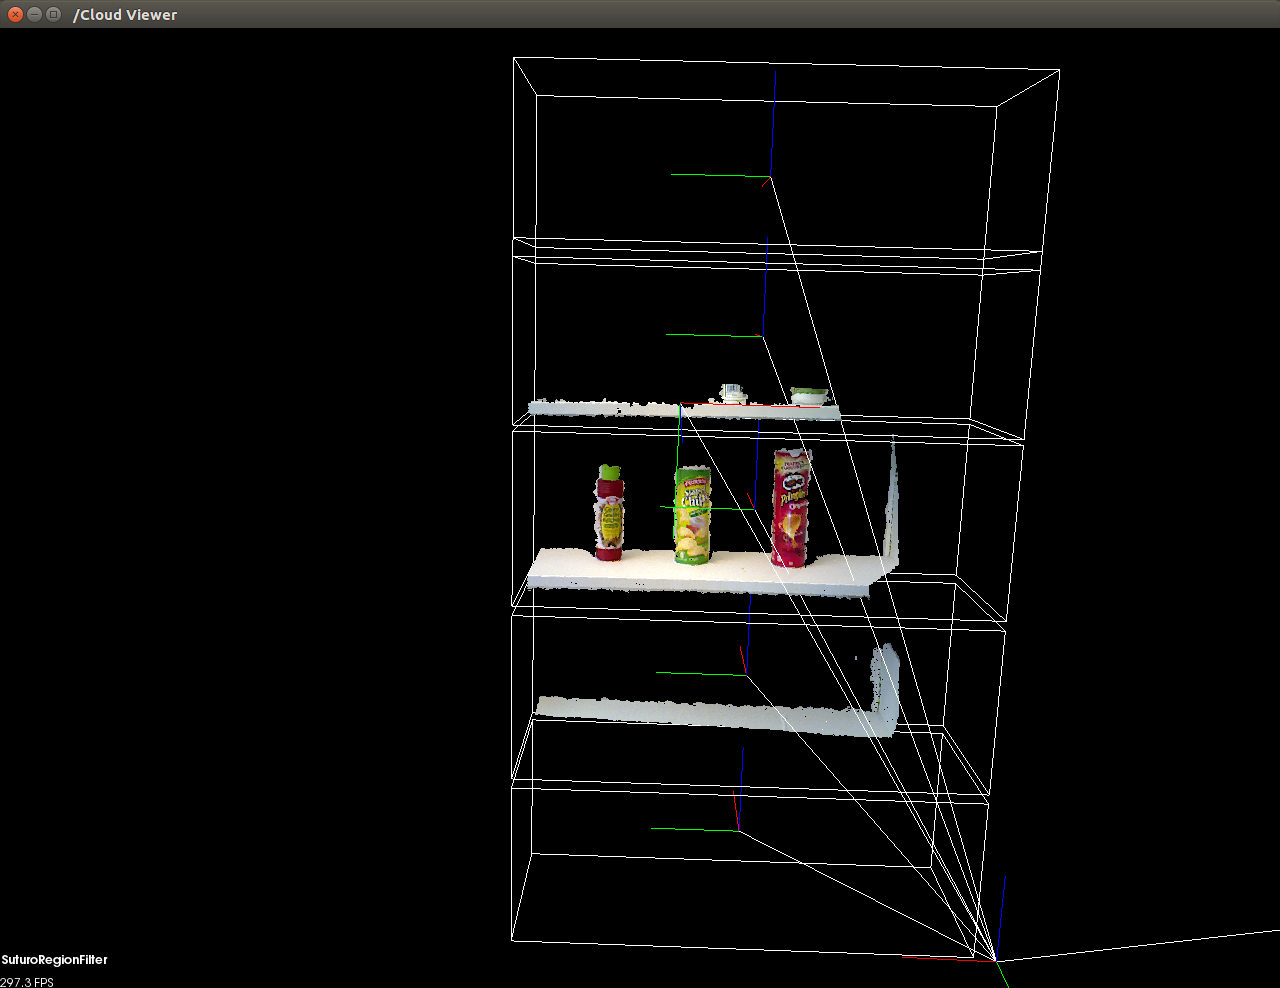
\includegraphics[width=0.5\textwidth]{pictures/pcl/RegionFilter.png}
        }\\ %  ------- End of the first row ----------------------%
        \subfigure[NormalEstimator]{%
            \includegraphics[width=0.5\textwidth]{pictures/2d/NormalEstimator.png}
        }%
        \subfigure[NormalEstimator]{%
           \includegraphics[width=0.5\textwidth]{pictures/pcl/NormalEstimator.png}
        }\\ %---End row----
        \subfigure[PlaneAnnotator]{%
            \includegraphics[width=0.5\textwidth]{pictures/2d/PlaneAnnotator.png}
        }%
        \subfigure[PlaneAnnotator]{%
           \includegraphics[width=0.5\textwidth]{pictures/pcl/PlaneAnnotator.png}
        }
\caption{hsrb\_1ms pipeline (1)}

\end{figure}
\newpage
\begin{figure}[H]
\centering
        \subfigure[PointCloudClusterExtractor]{%
            \includegraphics[width=0.5\textwidth]{pictures/2d/PointCloudClusterExtractor.png}
        }%
        \subfigure[PointCloudClusterExtractor]{%
            \includegraphics[width=0.5\textwidth]{pictures/pcl/PointCloudClusterExtractor.png}
        }\\%----------end row---------
        \subfigure[ClusterColorHistogramAnnotator]{%
            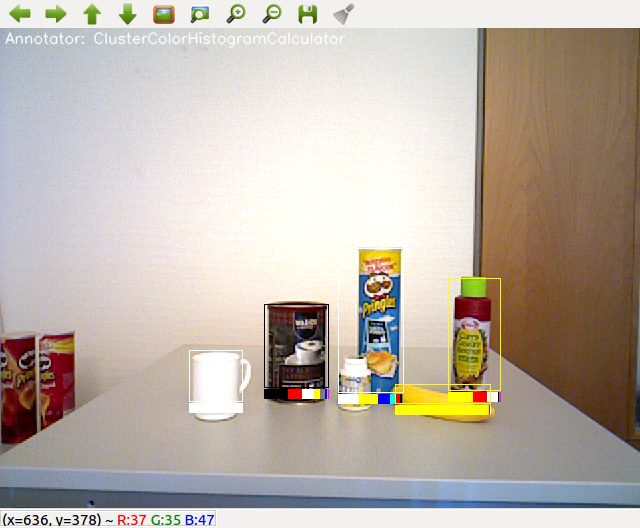
\includegraphics[width=0.5\textwidth]{pictures/2d/ClusterColorHistogramAnnotator.png}
        }%
        \subfigure[Cluster3DGeometryAnnotator]{%
          \includegraphics[width=0.5\textwidth]{pictures/2d/Cluster3DGeometryAnnotator.png}
        }\\ %  ------- End of the first row ----------------------%
        \subfigure[Cluster3DGeometryAnnotator]{%
            \includegraphics[width=0.5\textwidth]{pictures/pcl/Cluster3DGeometryAnnotator.png}
        }%
         \subfigure[PrimitiveShapeAnnotator]{%
           \includegraphics[width=0.5\textwidth]{pictures/2d/PrimitiveShapeAnnotator.png}
        }%
\caption{hsrb\_1ms pipeline (2)}
\end{figure}

\begin{figure}[H]
\centering
	\subfigure[PrimitiveShapeAnnotator]{%
            \includegraphics[width=0.5\textwidth]{pictures/pcl/PrimitiveShapeAnnotator.png}
        }%  ------- End of the first row ----------------------%
         \subfigure[SuturoShapeAnnotator]{%
           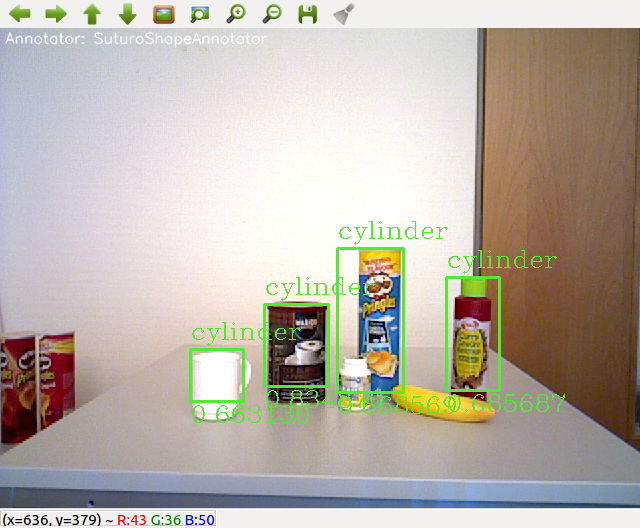
\includegraphics[width=0.5\textwidth]{pictures/2d/SuturoShapeAnnotator.png}
        }\\%
        \subfigure[KnnAnnotator]{%
            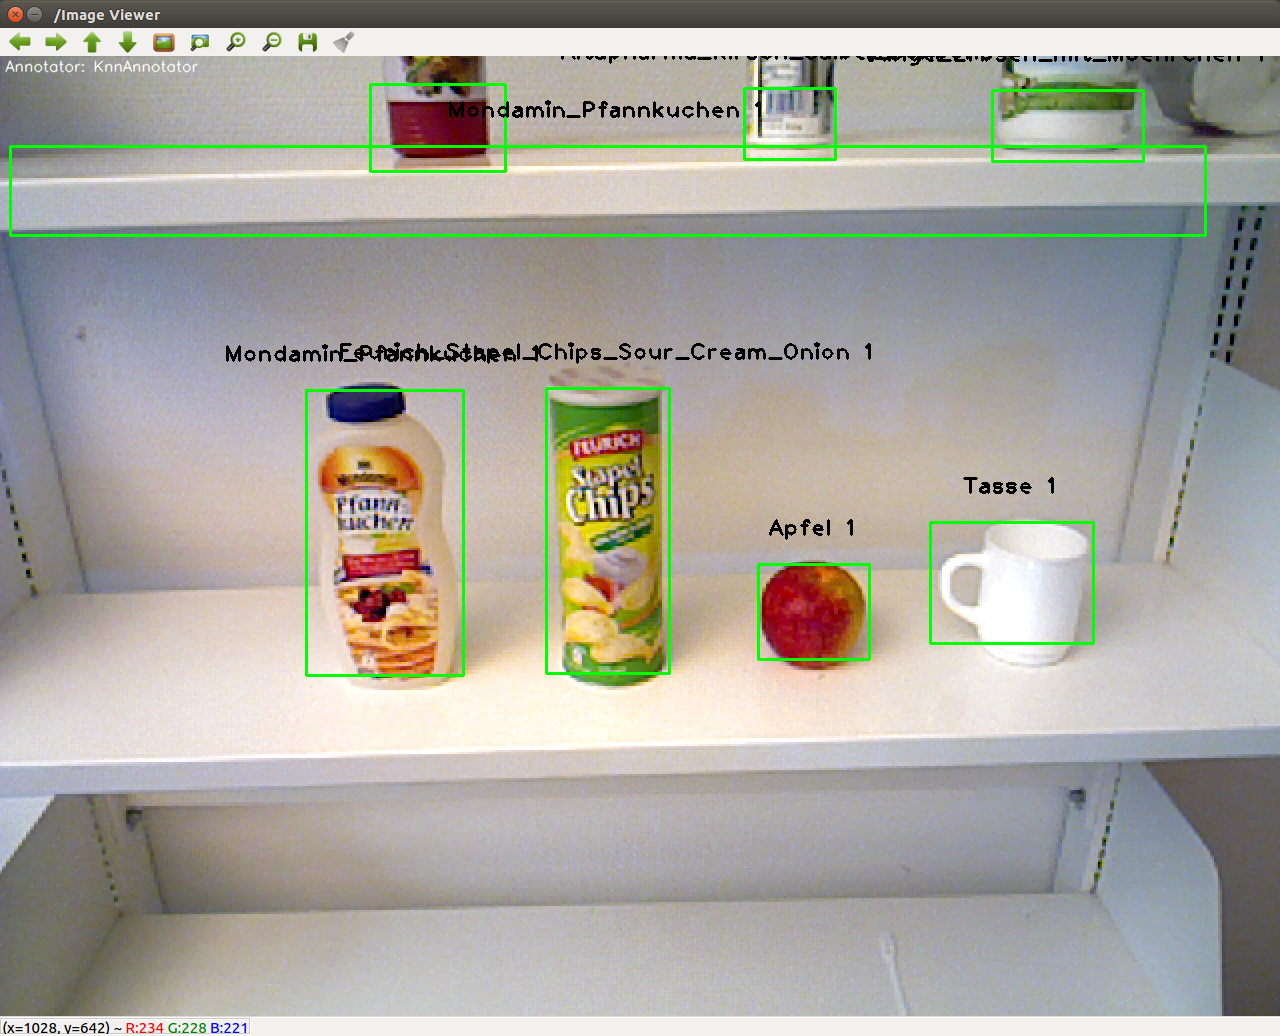
\includegraphics[width=0.5\textwidth]{pictures/2d/KnnAnnotator.png}
        }%
\caption{hsrb\_1ms pipeline (3)}
\end{figure}

			\subsection{Pipeline: hsrb\_planes} 
This pipeline is used to detect a shelf door. We try to find a plane that is parallel to the z-axis of the camera.
\begin{itemize}
	\item CollectionReader : Takes care of the camera input
	\item ImagePreprocessor : Implements image filters  
	\item PointCloudFilter : Filters points out of the cloud that are not in the range of the given parameters for X, Y and Z axes
	\item NormalEstimator : Estimate surface normal's in a PointCloud 
	\item PlaneAnnotator : Finds a plane in the current scene and saves it into the CAS.
	\item PointCloudClusterExtractor : Extracts all points that are found in the PointCloud that are perpendicular to the plane 
\end{itemize}

			\subsection{Pipeline: storage\_suturo} 
Pipeline for storing camera images in MongoDB, all saved scenes can be replayed for testing without the HSR and have the same functionality. 
\begin{itemize}
	\item CollectionReader : Takes care of the camera input
	\item ImagePreprocessor : Implements image filters 
	\item StorageWriterSuturo :  Records defined camera topics into the MongoDB
\end{itemize}

		\section{actionserver}
		\chapterauthor{Leonidas Paniago}
			\subsection{ExtractObjectInfoClient}
Call ExtractObjectInfoServer and wait until the result arrives or the time out runs out. Region can be set to limit the perception of objects to a specific region, if default is set the RegionFilter will be disabled. 

			\subsection{ExtractObjectInfoServer}
Receives a goal from ExtractObjectInfoClient and then SuturoProcessManager, checks for results and publishes them under perception\_actionserver/result. 

			\subsection{ExtractPlaneInfoClient}
Call ExtractPlaneInfoServer and wait until the result arrives or the time out runs out. This client has no additional parameters.

			\subsection{ExtractPlaneInfoServer}
Receives a goal from ExtractPlaneInfoClient and pass on to SuturoProcessManager, checks for result and publishes it under \texttt{perception\_actionserver\_plane/result}.

			\subsection{perception\_server}
Launches the \texttt{ExtractObjectInfoServer} and \texttt{ExtractPlaneInfoServer} and has no other functionality.

		\section{rs\_turn\_table}
		\chapterauthor{Leonidas Paniago}
rs\_turn\_table is a package from the last Suturo group. There were no big changes to the core code, only small situational changes not implemented on the master. 
This package is mainly for image recording, all recorded images will then be used for object recognition.  
			\subsection{Pipeline: estimate\_plane}
\begin{itemize}
	\item CollectionReader : Takes care of the camera input
	\item ImagePreprocessor : Implements image filters  
	\item PointCloudFilter : Filters points out of the cloud that are not in the range of the given parameters for X, Y and Z axes
	\item PlaneAnnotator : Finds a plane and saves it to a file 
\end{itemize}
This Pipeline will save all visible planes, they are callable again. The best way to get a clean plane is to set the Limits on PointCloudFilter by hand. Only one plane should be visible. 

			\subsection{Pipeline: save\_images}
\begin{itemize}
	\item CollectionReader : Takes care of the camera input
	\item ImagePreprocessor : Implements image filters  
	\item PointCloudFilter : Filters points out of the cloud that are not in the range of the given parameters for X, Y and Z axes
	\item NormalEstimator : Estimate surface normal's in a PointCloud 
	\item PlaneAnnotator : Finds a plane in the current scene and saves it into the CAS
	\item PointCloudClusterExtractor : Extracts all points that are found in the PointCloud that are perpendicular to the plane 
	\item SaveClusterCloudsAndImages : Save Information about the Cluster to a file 
\end{itemize}
Uses the saved plane and takes periodic images from objects on the plane, if there is more than one cluster visible the annotator will not trigger the saving process.

\section{classificationEvaluation Package}
\chapterauthor{Jan-Frederik Stock}

The classificationEvaluation package is used to save and display the classificationresults of the perception pipeline. The results can be saved in a markdown table and/or be displayed as a scatterplot. It consists mainly of the rsClassificationEvaluator.py python script. Here, the class ResultActionClient is implemented, which serves as an action client for the perception object info actionserver.\\

\subsection{The ResultActionClient class}
The class provides the following methods:

\begin{itemize}
\item 
sendGoal(self)\\
This method is used to send a goal to the ExtractObjectInfoServer and thus triggering the pipeline.

\item saveResult(self, result)\\
This method saves the actionresult, which is the classification, in a field of the class.

\item saveToMd(self, algorithm)\\
This method saves the collected results of the classification in a markdown table. If a markdown file with the name "evaluation.md" is found in the directory the script is executed in, the results are appended to it, otherwise, the file is created.

\item plotResult(self)\\
The method plots the collected results using the scatterplot function from matplotlib.
\end{itemize}

\subsection{Main method}
The main method tries to create an instance of the resultActionClient class, does some i/o with the user, sets the parameters for the resultActionClass, and then triggers the action. It also uses the provided methods to save the results to a markdown file and plot them.

\section{Feature Extraction Tools}
 \chapterauthor{Jan-Frederik Stock}
Perception uses feature extraction to get quantifiable data from the perceived images. On this data, the classification algorithms can then be trained. Every time a new image is perceived, its features are extracted, which are then used to classify it. Perception uses a neural network without the output layer to extract features, the output of this network are the features. The neural networking framework used for this is Caffe, the trained network is the BVLC Reference Net. The tools directory in the featureExtraction package contains the two bash scripts make\_split\_from\_directory.sh and make\_split\_list\_from\_directory.sh.

\subsection{make\_split\_from\_directory.sh} 
This bash script can be used to create a split YAML-file which is required to perform feature extraction with the rs\_addons package. To use it, one has to place the file in the parent directory of the directory, in which the folders with the recorded images are stored. When being executed, the script asks for a filename and the name of the directory out of which the YAML-file will be created. It then creates the YAML-file using the names of the directories in which the images are stored as class names.

\subsection{make\_list\_from\_directory.sh}
This bash script does nearly the same thing as the make\_split\_from\_directory.sh, except that it does not create a split file but a list of the class names. This is required by the classifying annotator and has to be pasted into the annotators YAML-file. The comma after the last class name in the list has to be removed manually.

\section{calculateConfidence in RSKNN.cpp}
\chapterauthor{Jan-Frederik Stock}
In the RSKNN.cpp, implementing KNN-classification in the rs\_addons package, the following method was added:

\begin{lstlisting}
double RSKNN::calculateConfidence(double classificationResult, cv::Mat neighborResponses)
\end{lstlisting}

It calculates the classification confidence for the KNN-classification by dividing the number of neighbors belonging to the result class, by the total number of visited neighbors. 

\section{The clusterLabeling Package}
\chapterauthor{Jan-Frederik Stock}
This package fixes a fundamental problem: Before its existence it was not possible to compare the performance of classifiers objectively. A very common procedure in machine learning is the evaluation of an algorithm by splitting the available data into a test set and a training set. The available data contains a class label for every sample.\\

The algorithm is trained on the training set and the test set is held back to test the performance. This is done by introducing samples from the test set into the algorithm and then checking if the algorithm produces the correct label. By dividing the number of correctly classified samples by the total number of tested samples, the accuracy is calculated. This is a very common measure of classification performance and it is suitable for a multi class problem like this.\\

The classification 

\subsection{Usage}

\subsubsection{The clusterLabelingAnnotator}
The clusterLabelingAnnotator is the Annotator used for labeling. It is best placed at the end of your labeling pipeline, which also has to contain the annotators necessary for clustering. The labeling and the evaluation work best if a good clustering is achieved, so it is recommended to use the PointCloudFilter or other filters you may have to ensure this. You mustn't change the settings of any annotator in the pipeline while creating the labels and using them for the evaluation later, otherwise, it can not be guaranteed that the cluster numbering will stay the same. To be able to label a scene frame by frame, put the Trigger at the beginning of your pipeline. You can use the classificationEval pipeline in the rs\_perception package to start.\\

To label a scene, you start your labeling pipeline and call the trigger service once. You can then chose the labelingAnnotator in the visualizer, which will display a number for every cluster.
\begin{center}
%Insert image
  %\includegraphics[width=\linewidth]{boat.jpg}
  %\caption{A boat.}
  %\label{fig:boat1}
\end{center}


Now, you can note the class for every cluster in a labeling JSON-file, look at the file already present in the labeling directory in the custerLabeling package for the correct syntax. Now call the trigger service again and proceed to label. If you do not want to create labels for a frame, for example if the clustering is bad, you can just leave the clusters array in the JSON-file empty. The classificationEvaluationAnnotator will leave this frame out of the calculation. Currently, one has to create the labeling JSON-file by hand, but there is a started implementation for a GUI for this task in the clusterLabeling package.

\subsubsection{classificationEvalutationAnnotator}
The classifcationEvaluationAnntator can read a labeling file and will then compare the labels with the actual classification to calculate the accuracy. Swap the classificationEvaluationAnnotator with the clusterLabelingAnnotator and add you classifying annotators before it. Do not change anything else about the pipeline. Set the path to your labeling file in the descriptor YAML-file of the classificationEvaluationAnnotator and start your pipeline. Trigger the pipeline as many times as you have labeled frames in your JSON-File. The classificationEvaluationAnnotator will display the current accuracy in your step in \textit{RoboSherlocks} terminal output. 

\subsection{Documentation}
\subsubsection{clusterLabelingAnnotator}
\begin{lstlisting}
TyErrorId processWithLock(CAS \&tcas, ResultSpecification const \&res_spec)
\end{lstlisting}
This is the main processing method of the annotator. It gets the detected clusters, draws a rectangle around their position, writes the number corresponding to their position in the clusters vector next to the rectangle, and then displays the new picture in the viewer.


\subsubsection{classificationEvaluationAnnotator}
\begin{lstlisting}
TyErrorId initialize(AnnotatorContext \&ctx)
\end{lstlisting}

This method is executed at the startup of the pipeline.  It gets the path to the labeling file from the YAML description and reads the file. The file is then parsed into a JSON object representation by rapidjson and saved in a field of the class.

\begin{lstlisting}
TyErrorId process(CAS \&tcas, ResultSpecification const \&res_spec)
\end{lstlisting}

This method loops through the identified clusters in a frame and compares the classification with the corresponding labels in the JSON-file for the frame. It then calculates the accuracy based on the comparison.



\section{rs\_hsrb\_perception Package}
\chapterauthor{Evan Kapitzke}

The \texttt{rs\_hsrb\_perception} package was created in the Suturo Master-project. The package implements a RoboSherlock process manager, called the \texttt{SuturoProcessManager}. Additionally, it contains modified annotators to annotate regions.

\subsection{RegionAnnotator}
\begin{itemize}
\item TyErrorId process(tcas, res\_spec)\\
Iterates through the clusters that are currently saved in the CAS and annotates the region in which they are presently based on the cluster pose.
This method only got changed to work with the \textit{RoboSherlock} master.
\end{itemize}

\subsection{SaveClusterCloudsAndImages}
Currently not used.

\subsection{SuturoClassifier}
Currently not used.

\subsection{SuturoProcessManager}
\begin{itemize}
\item setup()\\
Creates the ressource manager and instantiates the region vector.

\item init(pipeline)\\
Initializes the given pipeline (aggregate analysis engine YAML descriptor) and starts the visualizer.
This method got changed to allow the visualization of the pipeline.

\item run(args, detectionData)\\
Executes the initialized pipeline once with the given arguments and saves the result in detectionData.
This method now checks for the region "robocup\_default" and disables the region filter to perceive objects that can not be found
in a region. For example, a Pringles can that is placed on the ground.

\item has\_vertical\_plane()\\
Returns true if the current CAS contains a vertical plane.

\item getClusterFeatures(cluster, data)\\
Extracts the annotations of the given cluster and generates an ObjectDetectionData object. 
This object will be added to the data pointer. makeObjectDetectionData(...) from suturo\_conversion is used.
Currently only one KnnAnnotator (for known objects) is used to determine the class label of an object.

\item visControlCallback(req, res)\\
Callback for navigation through the different annotation previews in the visualization window.
\end{itemize}

\subsection{SuturoRegionFilter}
Adapted region filter from RoboSherlock.

\begin{itemize}
\item reconfigure()\\
Reconfigures the annotator to disable/enable its functionality without restarting the pipeline or removing it.
\end{itemize}

\subsection{suturo\_conversion}
Implements template functions to convert from and to PoseStamped objects.
Following functions got changed:

\begin{itemize}
\item decode\_shape(shapes)\\
Converts the result of the PrimitiveShapeAnnotator to match the required shape format in the ObjectDetectionData object.

\item makeObjectDetectionData(pose, geometry, shape, objClass, confidence, c, odd)\\
Combines the given parameters to an ObjectDetectionData message.
\end{itemize}

			\section{rs\_Athene}
			\chapterauthor{Leonidas Paniago De Oliveira Neto}
Handcamera\_tracking is the GitHub sub-branch containing rs\_Athene and all following featured annotators. 
None of them made it to the main branch because they were not finished or were not suitable for any current task.

				\subsection{TwoDAnnotator}
The TwoDAnnotator is responsible for shape recognition that should replace the old ShapeAnnotator by improving the accuracy, reducing processing time, and expanding the usability. 
Since the old annotator only processes RGB-D images (color and dense depth images) which makes the head-camera the only usable camera for the task. The task also takes a very long time with less than desirable results.
To fix these issues, the TwoDAnnotator uses only RGB (color images) images, which makes the processing less demanding than there's less data to process. Furthermore all the HSR cameras are usable for shape recognition because each one is capable of outputting RGB images.
The TwoDAnnotator works by converting the RGB image to grayscale then smoothing the grayscale output for better results and afterward running the canny-algorithm (openCV implementation). This provides all edges in the image which are used for the contour search, all found contours get examined for geometric shapes. 
During testing, it turns out that the Hough Circle Transform used to find circles is in the current form to slow. The whole annotator is way too unstable to be used in a real environment. It did not bring any improvement over the old ShapeAnnotator and need further work to be usable. 
In the end, this approach was no longer needed and was discarded. 

\begin{figure}[H]
\centering
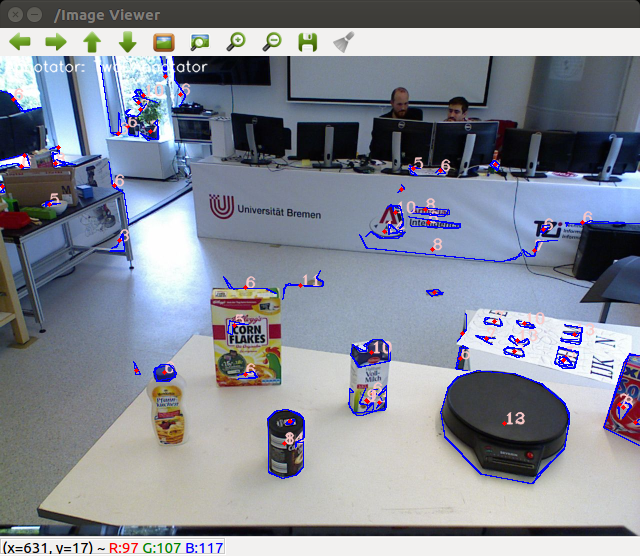
\includegraphics[width=1\textwidth]{pictures/perception/TwoDAnnotator.png}
\caption{TwoDAnnotator output example}
\end{figure}
				\subsection{YOLO}
The YOLO annotator is as the name suggests, an implementation for the You Only Look Once network. It contains all the needed code for the network to work.
But due to ROS not supporting openCV latest version there is no way to execute the annotator. It can be said that the algorithm will work if the supported version of ROS gets updated. Then a similar approach was utilized in the GoogLeNet annotator which succeeded and the created YOLO prototype worked like intended.
The approach is based on a python example and works by loading a pre-trained network and feeding it with RGB images. The output consists of all found classes and their bounding boxes that are over a set threshold.
In addition to classification the annotator calculated the distance from each bounding box center to the image center. Then the main focus for this annotator was, getting feedback on the current object position in relation to the camera center.

\begin{figure}[H]
\centering
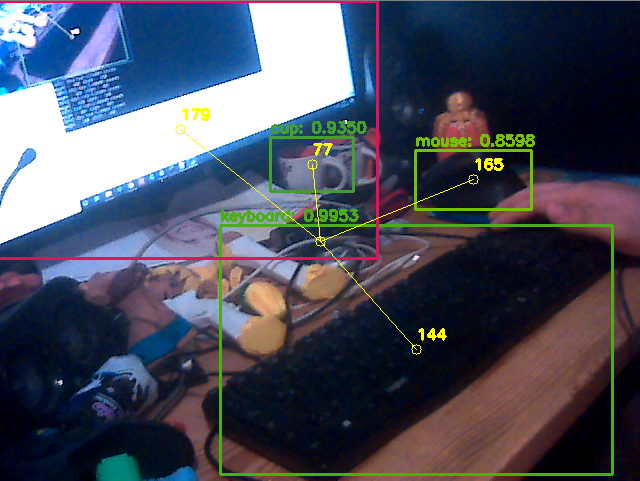
\includegraphics[width=1\textwidth]{pictures/perception/YOLO.png}
\caption{Python prototype output}
\end{figure}

				\subsection{GoogLeNet}
GoogLeNet is an annotator wich a similar approach to the YOLO annotator. Both networks use RGB images with the advantage that GoogLeNet runs on an older OpenCV version compatible with ROS.
The Robosherlock implementation uses the trained network to classify objects. The whole class structure is very similar to the YOLO annotator that OpenCV uses the same framework for all supported network architectures.
GoogLeNet differs from YOLO by only outputting the class probability so there is no information about where the classes are in the image. This makes the annotator useless for tracking objects, but can still be used for classification by extracting the classes with high probability.
Due to the output there is no visualization for this annotator.

				\subsection{PythonEmbedding}
PythonEmbedding annotator is an example of how a Python pure embedding (calling python script during runtime in c++) can be implemented in Robosherlock. The annotator converts the basic image container Mat to NumPy array. The script “Hello\_World.py” will then open and calls the only existing function “start”  using the image array as input, resulting in a new window with the sent image.
The current version of Robosherlock does not support Python annotators, Python pure embedding could represent an interim solution to this problem.

\endgroup
\end{document}

